%*****************************************
\chapter{Frequency Tables}\label{fre:frequency_tables}
%*****************************************
%TODO Reviewed

\section{Introduction}

Nominal and Ordinal data items are normally reported in frequency tables where the counts for a particular item are displayed. Crosstabs are a type of frequency table used to compare the counts of items that have been grouped in some way. This lab explores both frequency tables and crosstabs.

\section{Frequency Tables}

A frequency table simply lists a count of the number of times that some nominal or ordinal data item appears in a dataset. These types of tables are common around election time when polls report the number of people who voted for or against some proposition. As an example, here is a frequency table for the passenger rating in the \textit{cars} dataset.

\begin{figure}[H]
  \begin{center}
    \fbox{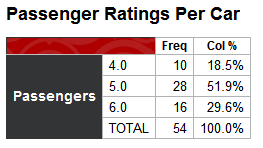
\includegraphics[]{gfx/fre005}}
    \caption{Passenger Ratings Per Car}
  \end{center}
\end{figure}

The above table shows that $ 10 $ cars in the dataset were rated for four passengers, $ 28 $ for five passengers, and $ 16 $ for six passengers, for a total of $ 54 $ rated cars. The table also shows the various row percentages so the researcher could report that $ 18.5\% $ of the cars were rated for four passengers.

A second example of a frequency table was created from the \textit{email} dataset. This frequency table shows the number of images that were attached to messages.

\begin{figure}[H]
  \begin{center}
    \fbox{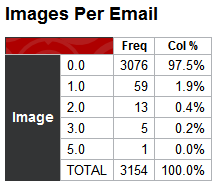
\includegraphics[]{gfx/fre010}}
    \caption{Images Per Message}
    \label{fre:img02}
  \end{center}
\end{figure}

Figure \ref{fre:img02} shows that $ 97.5\% $ of $ 3154 $ email messages contained no images while a small number of messages contained one or more images.

Frequency tables are only useful for nominal or ordinal data-type items. To illustrate why this is true, imagine creating a survey for all of the students at the University of Arizona and including ``age'' (interval-type data) as one of the survey questions. Attempting to create a frequency table for the ages of the respondents would have, potentially, more than $ 65 $ rows since student ages would range from about $ 15 $ to more than $ 80 $ and each row would report the number of students for that age. While a frequency table that large could be created it would have so many rows that it would be virtually unusable.

\section{Crosstabs}

A crosstab (sometimes called a contingency table or pivot table), is a table of frequencies used to display the relationship between two nominal or ordinal variables. These are commonly used around election time when pollsters create tables that show things like the number of people who voted for or against some proposition counted by gender, race, or some other factor. As an example of a crosstab, consider the following from the \textit{email} dataset.

\begin{figure}[H]
  \begin{center}
    \fbox{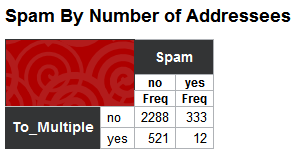
\includegraphics[]{gfx/fre015}}
    \caption{Addressees As A Function of Spam}
    \label{fre:img03}
  \end{center}
\end{figure}

In Figure \ref{fre:img03} notice that $ 2288 $ messages were sent to a single addressee and were identified as not spam while $ 521 $ messages were sent to multiple addressees and identified as not spam. By using a crosstab, a researcher can determine the frequency of some incident (email messages) by two different criteria (spam and multiple addressees). 

Here is a second example from the \textit{email} dataset:

\begin{figure}[H]
  \begin{center}
    \fbox{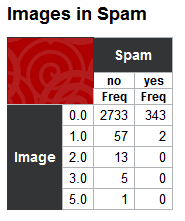
\includegraphics[]{gfx/fre020}}
    \caption{Images As A Function of Spam}
    \label{fre:img04}
  \end{center}
\end{figure}

In Figure \ref{fre:img04} notice that spam in general has no images. In fact, only two email messages out of $ 345 $ had one image, and no messages had more than one.

\subsection{Complex Crosstabs}

It is possible to create crosstabs that are quite complex, with multiple subcategories for both rows and columns. However, these tables are often too complex to be easy to interpret. Consider the table in Figure \ref{fre:img05}.

\begin{figure}[H]
  \begin{center}
    \fbox{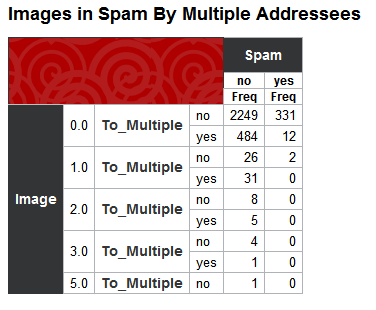
\includegraphics[]{gfx/fre025}}
    \caption{Images and Addressees As A Function of Spam}
    \label{fre:img05}
  \end{center}
\end{figure}

In the crosstab presented, $ 2249 $ email messages were identified as not spam, had zero images, and went to a single addressee. While this crosstab presents a lot of data in a compact form it is difficult to read and make sense of any one data cell. In general, it is preferable to have only one variable for both the rows and columns in a crosstab.

\section{Procedure}

\subsection{Frequency Table}

Start \texttt{SOFA} and select ``Report Tables.'' Then:

\begin{enumerate}
  \item Data Source Table: email
  \item Table Type: Frequencies
  \item Rows: Format
  \item Title: Types Of Email Messages
  \item Row Config: Check ``Total''
  \item Column Config: Check ``Frequency'' and ``Column \%''
  
  \begin{figure}[H]
    \begin{center}
      \fbox{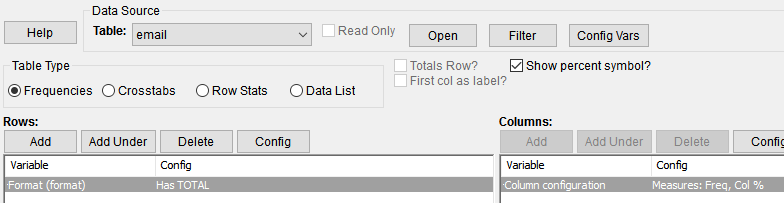
\includegraphics[width=0.95\linewidth]{gfx/fre030}}
      \caption{Setting Up Email Frequency Table}
    \end{center}
  \end{figure}

  \begin{figure}[H]
    \begin{center}
      \fbox{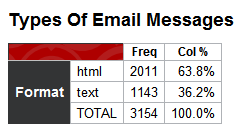
\includegraphics[]{gfx/fre035}}
      \caption{Email Frequency Table}
    \end{center}
  \end{figure}

\end{enumerate}

\subsection{Activity 1: Frequency Table} \label{fre:act01}

Using the \textit{maincafe} dataset in \texttt{SOFA}, produce a frequency table for Meal. The table should include both frequency and percentage for each of the four types of meals. The table should have a title of ``Frequency Tables, Activity 1'' and a subtitle of ``Frequency Table for Types of Meals''.

\subsection{Crosstabs}

Start \texttt{SOFA} and select ``Report Tables.'' Then:

\begin{enumerate}
  \item Data Source Table: births
  \item Table Type: Crosstabs
  \item Rows: Habit
  \item Columns: Premie
  \item Title: Premature Births By Habit
  
  \begin{figure}[H]
    \begin{center}
      \fbox{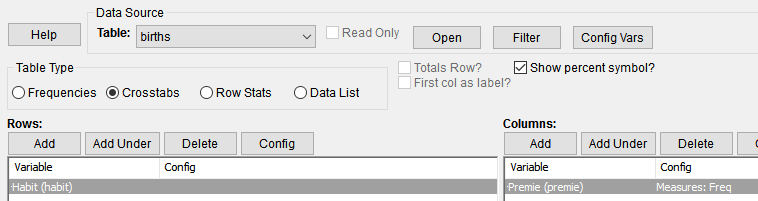
\includegraphics[width=0.95\linewidth]{gfx/fre040}}
      \caption{Setting Up Premature Births By Habit}
    \end{center}
  \end{figure}

  \begin{figure}[H]
    \begin{center}
      \fbox{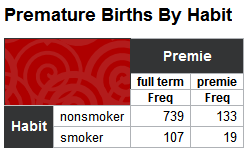
\includegraphics[]{gfx/fre045}}
      \caption{Premature Births By Habit}
    \end{center}
  \end{figure}
  
\end{enumerate}

To create a more complex crosstab, follow the instructions above for a simple crosstab but then click ``Add Under'' for Rows and select ``Mature.'' 

\begin{figure}[H]
  \begin{center}
    \fbox{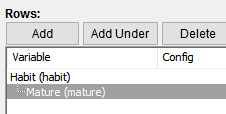
\includegraphics[]{gfx/fre050}}
    \caption{Setting Up Premature Births By Habit and Maturity}
  \end{center}
\end{figure}

\begin{figure}[H]
  \begin{center}
    \fbox{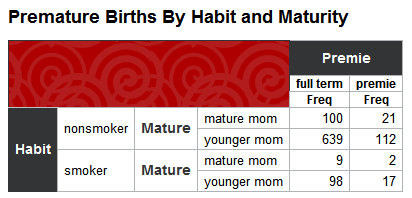
\includegraphics[]{gfx/fre055}}
    \caption{Premature Births By Habit and Maturity}
  \end{center}
\end{figure}

\subsection{Activity 2: Crosstabs} \label{fre:act02}

Using the \textit{maincafe} dataset in \texttt{SOFA}, produce a crosstab with the rows being Food and the columns being Svc. The crosstab should include only frequency and have a title of ``Frequency Tables, Activity 2'' and a subtitle of ``Crosstab for Food and Service''.

\subsection{Activity 3: Complex Crosstabs} \label{fre:act03}

Using the \textit{maincafe} dataset in \texttt{SOFA}, produce a crosstab with the rows being Pref with a sub-group of Sex and the columns being Meal. The crosstab should include only frequency and should have a title of ``Frequency Tables, Activity 3'' and a subtitle of ``Crosstab of Preference by Sex and Meal''.

\section{Deliverable}

Complete the following activities in this lab:

\rowcolors{1}{gray!25}{}
\begin{center}
  \begin{tabular}{lll}
    \hline 
    \textbf{Number} & \textbf{Name} & \textbf{Page} \\ 
    \hline 
    \ref{fre:act01} & \nameref{fre:act01} & \pageref{fre:act01} \\ 
    \ref{fre:act02} & \nameref{fre:act02} & \pageref{fre:act02} \\ 
    \ref{fre:act03} & \nameref{fre:act03} & \pageref{fre:act03} \\ 
    \hline 
  \end{tabular} 
\end{center}

Consolidate the responses for all activities into a single document and submit that document for grading.






